\documentclass[12pt, a4paper, oneside]{book}
 
% - taille de la fonte    : 10pt, 11pt, 12pt
% - recto ou recto-verso    : oneside, twoside
 
% Chargement d'extensions
\usepackage[utf8]{inputenc}    
\usepackage[francais]{babel}    
\usepackage[margin=1in]{geometry}
\usepackage{hyperref}
\usepackage{graphicx}
\usepackage{caption}
\usepackage{subcaption}
\usepackage{eurosym}
\usepackage{float}

% Informations le titre, le(s) auteur(s), la date
\title{La Blockchain}
\author{ Jordan Sagnes, Alexandre Ludwig, Yoan Fath, \\ Julien Pignolet et Arnaud Couderc}
\date{\today}
 
\begin{document}
 
\maketitle
 
    % Le prologue du livre
    \frontmatter
    %\section{Introduction}
 
    % Corps du livre
    \mainmatter
 
    % \chapter{Blockchain point de vue global}
    % \section{Un chapitre}
    % \subsection{Une subsection}
    % \subsubsection{Une sous-subsection}
    % \subsubsection{Une sous-sous-subsection}
    % On écrit ici}

    \chapter{Les applications de la blockchain}

    Majoritairement, lorsqu’on parle de blockchain, le premier mot qui nous vient à l’esprit est bitcoin. Peut-être à juste titre, car les cryptomonnaies représentent l’application la plus médiatisée de la blockchain. Mais saviez-vous que le domaine de la Finance n’est pas le seul à être courtisé par la blockchain ? Nous avons choisi de vous parler d’applications plus à la marge, qui pourraient révolutionner leurs domaines.

    \section{L'industrie du jeu video}

    Il y a une large variété d’implémentation possible de la blockchain dans le domaine du jeu vidéo~\cite{JV}, au-delà de l’utilisation de cryptomonnaies pour les microtransactions.  L’aspect infalsifiable du registre de transaction pourrait permettre aux jeux vidéo de se prémunir de la triche.
    \\
    C’est dans la gestion de la progression du joueur que la blockchain pourrait intervenir. En effet, la valeur d’un joueur est souvent associée à la quantité de pièces et d’objets brillants qu’il a pu acquérir en complétant des niveaux, succès, etc... La progression représente la colonne vertébrale de la plupart des jeux et sécuriser celle-ci, en la rendant infalsifiable, semble donc essentiel.
    \\
    Un exemple concret est Miniclip’s 8-Ball Pool. Il s’agit d’un jeu mobile de billard, où quelques joueurs ont réussi acquérir des avantages beaucoup plus tôt que prévu dans le jeu, leur donnant ainsi un avantage déloyal face aux joueurs honnêtes décourageant ces derniers de jouer.
    
    \begin{figure}[H]
        \begin{center}
          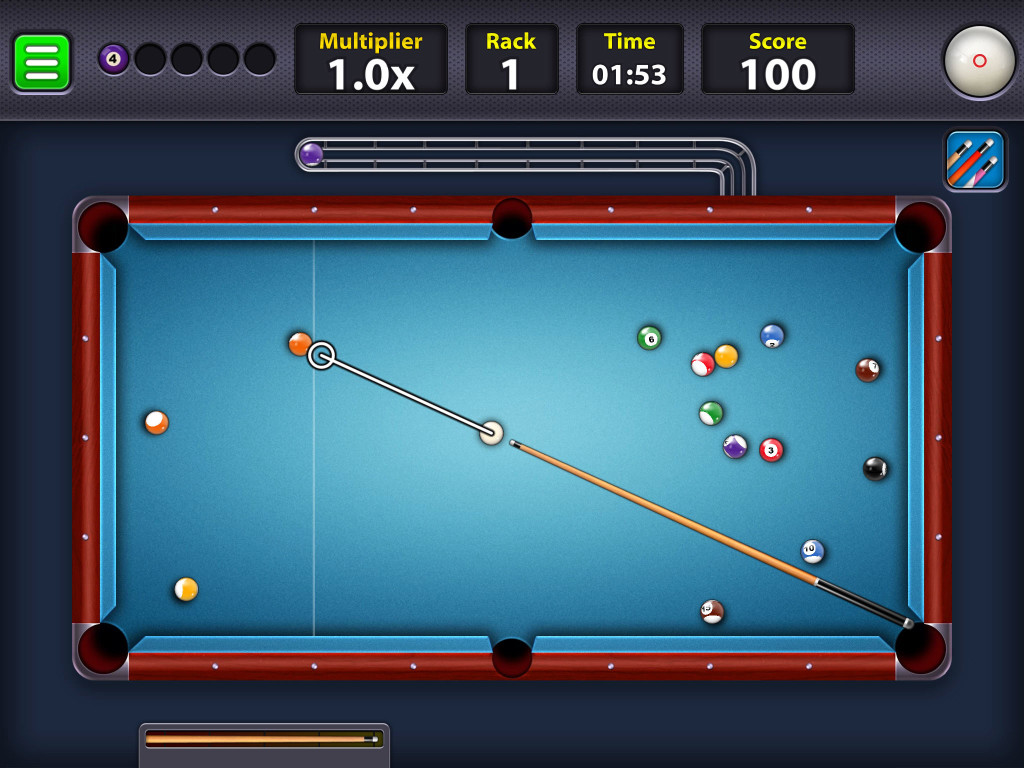
\includegraphics[width=.43\textwidth]{images/billard.jpg}
          \label{fig:chaine}
          \caption{Miniclip’s 8-Ball Pool : Un jeu mobile qui pourrait utiliser la blockchain}
        \end{center}
    \end{figure}

    Il semblerait que le géant Ubisoft~\cite{ubi} soit en train de mettre en place ce genre de solution.

    \section{L'industrie agroalimentaire}

    En parlant de géants, dans un tout autre domaine cette fois, Carrefour et Nestlé ont eux aussi adoptés la blockchain en s’alliant à IBM et sa solution IBM Food Trust~\cite{IBMfood}.
    \\
    Le postulat de base est simple. Les consommateurs n’ont jamais eu autant de choix dans la diversité de leurs aliments. Pourtant d’après IBM, 84\% des acheteurs considèrent au moment de leur achat, où et comment ont été produits les aliments. C’est là que la blockchain peut être décisive dans un milieu aussi compétitif puisqu'elle permet une transparence totale de la chaîne d’approvisionnement et de la fabrication, toujours grâce à l’aspect infalsifiable du registre de transaction.
    \\
    D’après Nestlé, cela permet de « renforcer le lien de confiance avec ses consommateurs ». C’est pourquoi ces derniers appliquent cette solution sur 15 de leurs produits phares, notamment la purée Mousline. Carrefour compte quant à lui déployer cette solution d’ici 2020 sur l’ensemble des produits alimentaires Filière Qualité Carrefour, soit 300 références.
    \\
    Assurer la traçabilité des produits représente aussi un avantage majeur en cas d’incident de sécurité alimentaire. Certaines compagnies, prennent parfois plusieurs jours à plusieurs semaines pour retracer leur propre chaine.
    \\
    En généralisant, la plus grosse vulnérabilité de la chaîne d’approvisionnement est le manque de transparence car c'est une porte ouverte vers la fraude et la corruption (exemple de la fraude sur l’étiquetage faisant passer de la viande de cheval pour de la viande de bœuf), problème qui est résolu par la blockchain.

    \section{Les Smart Contracts}
    Les smart contracts constituent l’un des types d’usage les plus prometteurs de la blockchain.


    \chapter{Blockchain dans sa technique}
    \section{Introduction}
    Nous allons illustrer le fonctionnement de la blockchain avec un exemple : Alice, Bob et Eve qui souhaite mettre en place une méthode sécurisée pour gérer leur argent ainsi que leurs transactions.

    \section{Qu'est-ce que la blockchain ?}
    Imaginons un livre dans lequel nous pouvons tout noter. Dans notre exemple, Alice pourra alors y indiquer le montant disponible sur son compte et toutes ses transactions réalisées. Une fois qu’une page est remplie, nous passons simplement à la page suivante.
    \\
    La blockchain fonctionne sur ce même principe sauf qu’en réalité les pages sont appelées des blocs, et qu’une fois le nombre de transaction maximal atteint, nous ouvrons un nouveau bloc.

    \section{Fonctionnement de la blockchain}
    \subsection{Intégrité d'un bloc}
    Il est important que toutes les données stockées dans la blockchain soient intègres, c’est-à-dire qu’il faut être sûr qu’elles n’aient pas été modifiées maladroitement ou par un utilisateur mal intentionné.
    \\
    Mettons en place notre exemple :
    \begin{enumerate}
        \item Alice, Bob et Eve possèdent tous 10 \euro~sur leur compte et n’ont encore effectué aucune transaction.
        \item Il n'y a aucune mesure de sécurité en place, Eve décide de modifier les données et de voler de l’argent à Alice.
    \end{enumerate}

    \begin{figure}[H]
        \centering
        \begin{subfigure}{.5\textwidth}
          \centering
          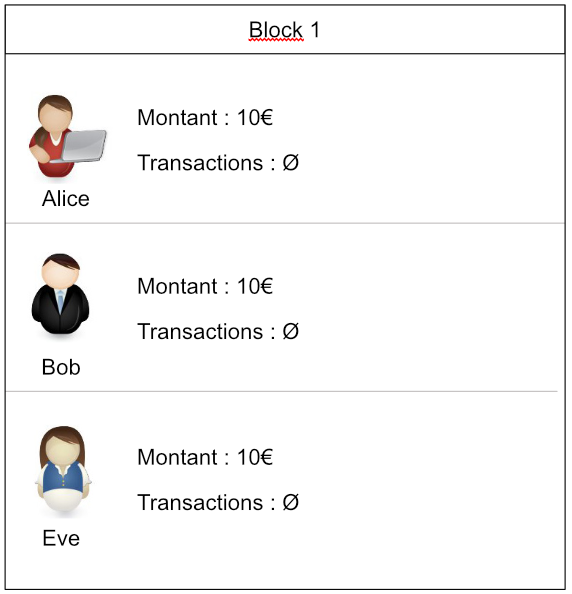
\includegraphics[width=.7\textwidth]{images/bloc1.png}
          \label{fig:bloc1}
        \end{subfigure}%
        \begin{subfigure}{.5\textwidth}
          \centering
          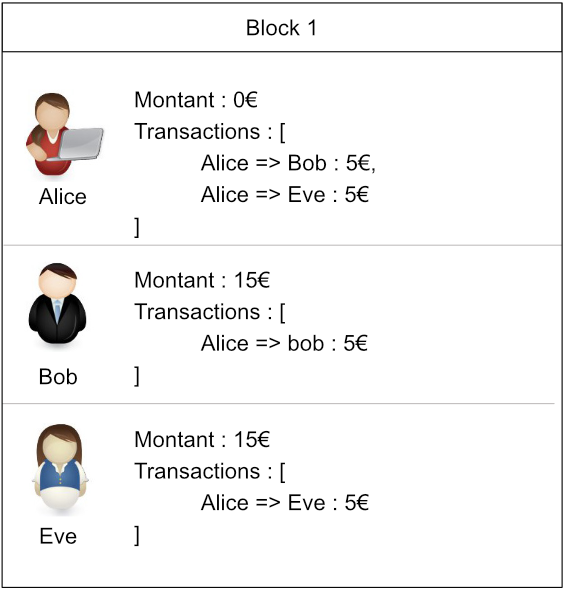
\includegraphics[width=.7\textwidth]{images/bloc2.png}
          \label{fig:bloc2}
        \end{subfigure}
        \caption{Le livre est ouvert, n'importe qui peut faire n'importe quoi.}
        \label{fig:test}
    \end{figure}

    Pour remédier à ce problème, une première solution est de hacher le contenu d’un bloc et d’inscrire le résultat dans celui-ci, or un hachage est très rapide à réaliser et donc rien ne pourrait empêcher Eve de modifier les données puis recalculer un nouveau hash. Une modification des informations présentes dans un bloc est donc nécessaire :

    \begin{itemize}
        \item En plus des informations déjà présentes, nous avons maintenant le hash du bloc précédent et le hash du bloc actuel : Pour l’obtenir nous hachons la totalité des informations, les transactions, le fichier nonce et le hash du bloc précédent.
        \item Un nonce est un fichier généré aléatoirement pour que le hash du bloc suive une règle précise (ici commencer par cinq zéros consécutifs). Nous reviendrons plus précisément sur ce sujet dans la partie Proof Of Work.
    \end{itemize}

    \begin{figure}[H]
        \begin{center}
          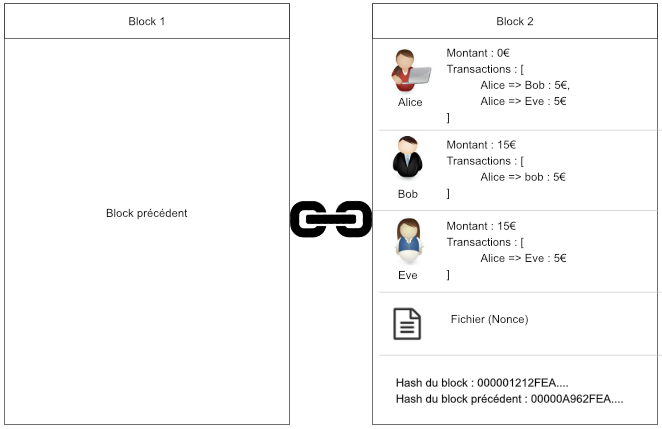
\includegraphics[width=\textwidth]{images/chaine.png}
          \label{fig:chaine}
          \caption{Une chaine de bloc : un bloc est lié à son prédecesseur par le hash de ce dernier.}
        \end{center}
    \end{figure}

    Maintenant, si Eve tente de modifier les données d’un bloc, il faudra qu’elle régénère le fichier nonce pour que le hash suive toujours la règle imposée, or cette opération est impossible à réaliser pour une seule personne car le nombre d’opérations à effectuer est très élevé. De plus si jamais Eve arrive par chance à en trouver un nouveau il faut qu’elle recommence pour tous les blocs suivants car elle devra modifier le hash du bloc précédent.

    \subsection{Intégrité du contenu d’un bloc}

    Dans la partie précédente nous avons vu comment nous assurer que les blocs sont intègres. Mais comment savoir avant d’ajouter des transactions dans un bloc que celles-ci n’ont pas été modifiées ?
    \newline
    Pour cela nous allons utiliser un arbre de Merkle, il s’agit d’un arbre de hachage binaire, son but est donc de vérifier l’intégrité d’un groupe de données (ici des transactions) sans devoir nécessairement utiliser toutes les données disponibles dans un bloc.

    \begin{figure}[H]
        \begin{center}
          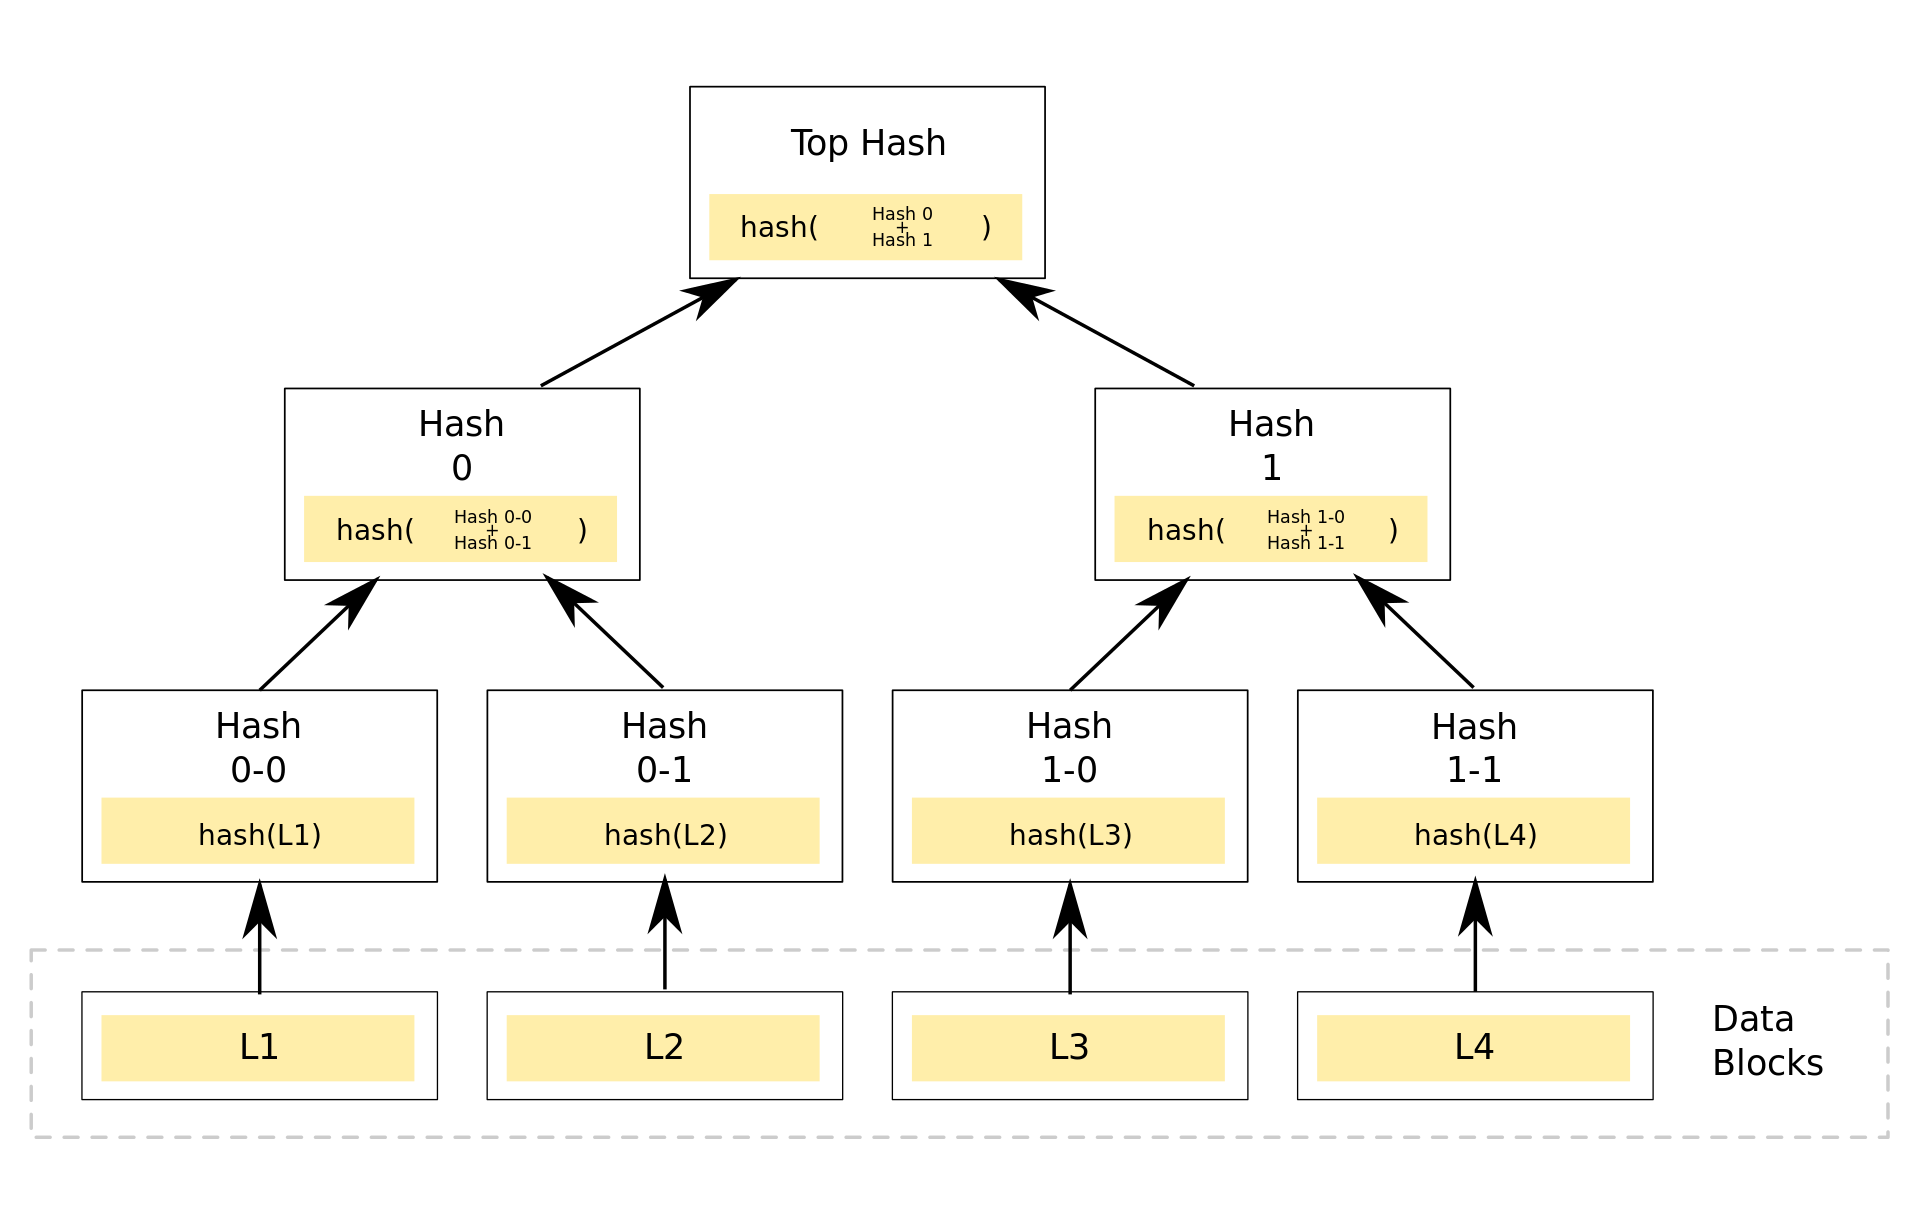
\includegraphics[width=\textwidth]{images/arbre.png}
          \label{fig:arbre}
          \caption{Un arbre de Merkle appliqué à la blockchain.}
        \end{center}
    \end{figure}

    Sur le schéma ci-dessus et en considérant que nous sommes encore dans notre exemple :

    \begin{itemize}
        \item Les feuilles (Hash 0-0, Hash 0-1, …) représentent le hash des transactions
        \item Leur parent représente la concaténation de leur hash et ainsi de suite
        \newline
    \end{itemize}
    Si nous vonlons vérifier l’intégrité de la transaction L3 (Hash 1-0), nous devons seulement posséder le hash de son frère (Hash 1-1), celui de son oncle (Hash 0) et enfin la racine (le Top Hash).
    \\
    Pour cette opération nous devons seulement être sûr de l’intégrité du « Top Hash », c’est pourquoi cette information sera rajoutée au contenu d’un bloc dont l'intégrité a été prouvée dans le point précédent.\cite{merkle}

    \newpage

    \subsection{Disponibilité de la blockchain}

    \subsection{Proof-of-Work}

    Le Proof of Work (PoW ou preuve de travail) est plus communément appelé minage. Les utilisateurs (Alice, Bob et Eve) disposent donc chacun d’une copie de la blockchain et ils ont différentes missions :

    \begin{itemize}
        \item Vérifier l’intégrité des blocs et des transactions : Ces opérations sont très rapides il s’agit simplement de vérifier les hashs.
        \item Créer / ouvrir des nouveaux blocs : Comme nous l’avons vu précédemment cette opération consiste à trouver un fichier « nonce » afin que le hash du bloc respecte certaines règles et donc sécuriser la blockchain. Cela prend énormément de temps de calcul et par conséquent provoque un réel impact écologique (électricité).
        \newline
    \end{itemize}

    Lorsqu’un mineur trouve un nonce correct, il le diffuse sur le réseau, les autres mineurs vérifient ce fichier et selon sa validité le mineur est alors récompensé, en effet il va percevoir tous les frais de transactions du bloc.

    \chapter{Les failles / types d'attaques + exemples connus}
    La blockchain n'est pas inviolable, mais comme souvent, les failles présentes sont dûes à des erreurs d'implémentations ou à des négligences. La seule attaque ne se basant pas sur ces vulnérabilités est appelée \emph{Attaque 51}.
    \section{Attaque 51}
    La blockchain se basant sur le principe de consensus, si un groupe de personne possède plus de 50 \% de la capacité de calcul, elle crée un autre consensus qui peut être faussé par l'introduction de blocs corrompus qui annuleraient des transactions par exemple. De ce fait, on peut modifier la blockchain et la faire plus longue que celle calculée par le reste du réseau, ce qui la rendrait légitime par tout le réseau.
    \subsection{Réalisation}
    Pour obtenir 51 \% de la puissance totale de calcul, on pourrait détourner des machines de calcul existantes pour les réunir sous une même banière (un même pool).
    Il existe également la possibilité de créer une nouvelle capacité de calcul, en créant une nouvelle ferme de serveur pour arriver à une capacité X+1 (avec X la capacité déjà existante) pour atteindre une capacité totale de X+X+1. Cette possibilité est seulement théorique puisqu'il faudrait doubler le parc existant, déjà colossal.
    \subsection{Finalité}
    Le but principal d'une attaque 51\% est de falsifier les blocs, pour masquer des transactions, falsifier des informations ou, dans le cas d'une cryptomonnaie, effectuer une double dépense, c'est-à-dire effectuer une transaction, l'effacer de la chaine, et effectuer une autre transaction à la place de la première.
    \newline
    Tout ceci peut casser la confiance dans une blockchain et la rendre caduque.
    \subsection{Exemple}
    En début d'année 2019, la blockchain Ethereum Classic (ETC) a subi une attaque 51, il y a eu plusieurs réorganisations, qui ont prmis des doubles dépenses. Le préjudice est éstimé à 219 500 ETC, soit plus de 1 million de dollars à l'époque.
    \\
    Cette attaque a été rendue possible car la puissance de calcul nécessaire était tellement négligeable que cela ne coutait que 4500 \$ par heure.\cite{51ETC}

    \section{Le naufrage \emph{The DAO}}

    

    \chapter{Point de vue légalité}
    \section{La blockchain et la protection des données}
    \subsection{L'incompatibilité avec la RGPD}
    Le droit des données personnelles permet 
    à une personne concernée de demander l’accès, la rectification 
    et l’effacement de ces données sous certaines conditions. 
    Si les blockchains privées permettent techniquement de gérer
    ces demandes par l’intermédiaire d’un contrat,
    le registre des blockchain publiques est immuable. De ce fait,
    une donnée personnelle inscrite par un tiers ne pourra pas être retirée 
    à la demande de l’utilisateur. Cette impossibilité entre en collision frontale avec le RGPD, 
    et notamment l’article 17 relatif au droit à l’effacement. 
    \\ 
    \newline
    Une solution à ce problème serait d'interdire l'usage de l'inscription de données personnelles dans la blockchain publique. 
    Cependant, cette solution de prend pas en compte les spécificités et les opportunités de la blockchain.
    \cite{reg}

    \subsection{Comment la blockchain protège notre vie privée ?}

    Malgré le fait que ses principes 
     soient incompatibles avec la RGPD, la blockchain apporte une protection à la vie privée non négligeable. 
     En effet, la blockchain est directement fondée sur des algorithmes de chiffrement robustes et sur le pseudonymat,
     ce qui la protège du hacking sans pour autant avoir besoin de collecte massive de données personnelles.
     \cite{reg}

    \section{Rapport d'activité de 2018 de l'ANSSI}

    Le 15 avril 2019, l'ANSSI a publié son rapport d'activités de 2018, intitulé \textit{"Construire ensemble la confiance 
    numerique de demain"}. 
    Dans ce rapport, L'ANSSI met en avant 5 types de cybermenaces, dont une qui viserait à générer de façon frauduleuse des 
    cryptomonnaies. Par conséquent, l'ANSSI considère que la sécurité absolue des blockchains n'est qu'un mythe.
    \cite{anssi2018}

    \section{La blockchain dans le Code monétaire et \\financier}

    En décembre 2017, Emmanuel Macron, afin de placer la France en tête de l'innovation financière en Europe, 
    a signé une ordonnance qui inscrit le droit d'utilisation de la blockchain dans l'investissement non-côté.
    \\
    \newline
    Ce projet modifie le Code Monétaire et financier de plusieurs manières. La première consiste à proposer la blockchain comme nouvelle 
    modalité technique d'inscription et de transfert des titres non côtés, à savoir les chapters de fonds, les titres de créance négociables,
    et les actions et obligations non côtés, qui devaient auparavant être matérialisé par un compte-titres.
    \\
    \newline
    Ils pourront désormais être inscris dans une blockchain puis être échangés sans passer par aucun intermédiaire.
    Par conséquent, cette technologie proposera une solution plus rapide, moins chère, plus transparente et plus sûre.
    \\
    \newline
    De plus, la France devient le premier pays européen et sûrement mondial à légaliser l'inscription et le transfert de titres non côtés par blockchain.
    \cite{CodeMonetaireFinancier}
 
    % Les annexes
    % \appendix
 
    % \section{Premier annexe}
    % \section{Second annexe}
 
    
    \backmatter
 
    % \section{Conclusion et discussion}
 
    
    \tableofcontents

    \bibliographystyle{unsrt}
    \bibliography{TD_SSI_biblio}
 
% Fin du document
\end{document}